\chapter{Rentabilidad, volatilidad y estadística}\label{cap:estadistica}

\section{Rentabilidades simples y logarítmicas}
La rentabilidad simple es $r_t = P_t/P_{t-1}-1$ y la logarítmica $\ell_t = \ln(P_t/P_{t-1}) = \ln(1+r_t)$.
Las logarítmicas \emph{suman en el tiempo} ($\ell_{0\to T} = \sum \ell_t$); las simples \emph{suman entre
activos} (la rentabilidad de una cartera es $\sum_i w_i r_i$). Usa la que convenga a cada cálculo y no
las mezcles.

Para precios que incluyen dividendos o cambios de contrato hay que usar series \textbf{ajustadas}
(capítulo~\ref{cap:commodities} para el roll de futuros); si no, aparecen saltos falsos.

\section{Volatilidad}
La volatilidad anualizada es la desviación típica de las rentabilidades escalada por la raíz del
número de periodos por año:
\begin{equation}
\sigma_{\text{anual}} = \sigma_{\text{diaria}}\sqrt{252},\qquad \sigma_{\text{diaria}}\approx \frac{\sigma_{\text{anual}}}{16}.
\end{equation}
La regla del 16 es útil: un activo con 32~\% de volatilidad anual se mueve en torno a un 2~\% diario
(una desviación típica). \py{trader.indicators.realized\_vol} calcula la volatilidad realizada en
ventana móvil; \py{trader.indicators.atr} la mide en unidades de precio (rango verdadero medio), que es
lo que se usa para colocar stops.

La volatilidad \textbf{no es constante}: se agrupa (periodos tranquilos y turbulentos), sube cuando los
precios caen en acciones (efecto apalancamiento) y revierte a la media. Por eso los traders
dimensionan con volatilidad reciente (EWMA, GARCH o ATR) y no con la de los últimos diez años.

\section{Colas gruesas}
Las rentabilidades reales tienen \textbf{colas mucho más gruesas} que la normal: movimientos de 5
desviaciones típicas, que bajo normalidad ocurrirían una vez cada varios miles de años, ocurren varias
veces por década. La figura~\ref{fig:colas} lo muestra con rentabilidades $t$ de Student ($\nu=4$).

\begin{figure}[h]\centering
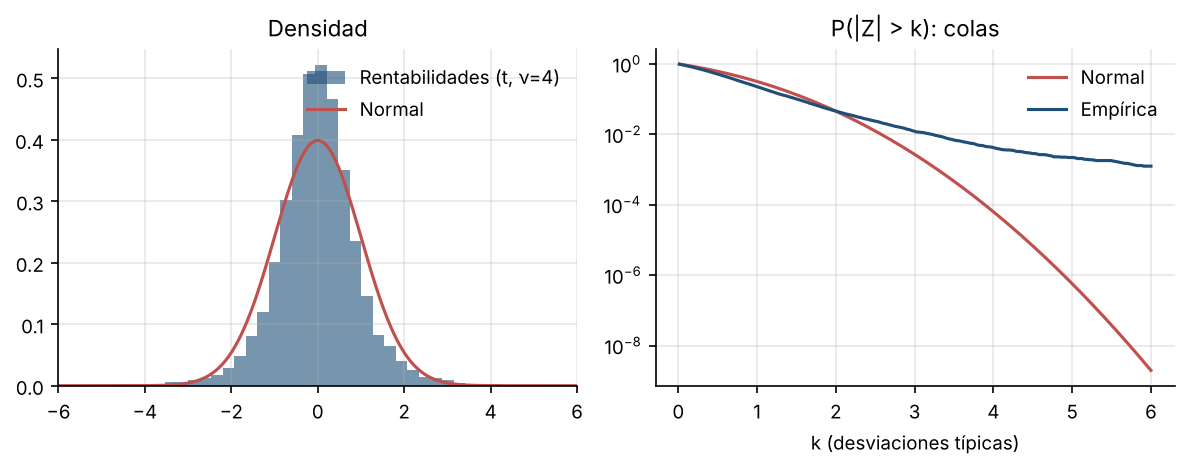
\includegraphics[width=\textwidth]{f02_colas}
\caption{Rentabilidades con colas gruesas frente a la normal. A la derecha, en escala logarítmica, la
probabilidad de superar $k$ desviaciones típicas: la diferencia es de órdenes de magnitud a partir de $k=4$.}
\label{fig:colas}
\end{figure}

\begin{aviso}
Cualquier medida de riesgo que asuma normalidad (VaR paramétrico, Sharpe, raíz del tiempo)
\textbf{infravalora} el riesgo de cola. Complementa siempre con escenarios de estrés y con el peor día
histórico (lo hace \py{scripts/informe\_riesgo.py}).
\end{aviso}

\section{Correlación}
La correlación entre activos es inestable y \textbf{tiende a 1 en las crisis}, justo cuando la
diversificación más se necesita. Diez posiciones en acciones tecnológicas no son diez apuestas: son
una apuesta con diez comisiones. Antes de abrir una posición, pregúntate qué otras posiciones de tu
cartera ganarían o perderían por el mismo motivo.

\section{Significación estadística}
Con rentabilidades i.i.d., el error estándar del Sharpe anual estimado con $n$ años es
aproximadamente $1/\sqrt{n}$. Con 4 años de datos, un Sharpe de 0,5 \textbf{no es distinguible de cero}
(error típico 0,5). Para afirmar con un 95~\% de confianza que un Sharpe de 1 es positivo hacen falta
unos 4 años; para uno de 0,5, unos 16. Esta aritmética simple explica por qué la mayoría de las
«estrategias ganadoras» son ruido (capítulo~\ref{cap:backtest}).

\begin{ejercicios}
\begin{enumerate}
\item Una acción tiene volatilidad implícita de 48~\%. ¿Cuánto se espera que se mueva en un día (1$\sigma$)?
  ¿Y en una semana?
\item Comprueba que $\ln(1{,}10)+\ln(1/1{,}10)=0$ pero $10~\%-9{,}09~\%\neq0$. ¿Qué implica para la media de rentabilidades simples?
\item Con \py{trader.data.synthetic\_ohlc} genera 20\,000 días y cuenta cuántos superan 4$\sigma$. Compara con la normal.
\end{enumerate}
\end{ejercicios}
